\documentclass[12pt, sumlimits, intlimits]{article}

\usepackage[utf8]{inputenc}
\usepackage[T1]{fontenc}
\usepackage[english]{babel}
\usepackage{hyperref}
\usepackage{lmodern, microtype}
\usepackage[top=3.5cm, bottom=2cm, right=2cm, left=3.5cm,
paper=a4paper]{geometry}
\usepackage[margin=2cm]{caption}
\usepackage{booktabs}
\usepackage{graphicx}
\usepackage{etoolbox}

\usepackage{amsfonts, amsmath, amssymb}
\usepackage{mathtools}
\newcommand \twopi{{{\scriptstyle(2}\mskip-2.0mu\pi{\scriptstyle)}}}
\newcommand \ee{{\mathrm e}}
\newcommand \ii{{\mathrm i}}
\newcommand \full{{\mathrm d}}
\newcommand \fulld[1]{{\frac \full{\full {#1}}}}
\newcommand \partiald[1]{{\frac \partial{\partial {#1}}}}
\newcommand \yesnumber{\addtocounter{equation}{1}\tag \theequation}

\usepackage{listings}
\lstset{basicstyle=\footnotesize\ttfamily, tabsize=2}

\usepackage[backend=bibtex, style=authoryear]{biblatex}
\addbibresource{refs.bib}

\setlength{\parindent}{0pt}
\setlength{\parskip}{2.5ex}
\pagenumbering{arabic}
\thispagestyle{empty}

\begin{document}


\includegraphics[width=8cm]{ecmi-logo.png}

ECMI Modeling Week 2018 \\*
University of Novi Sad, Faculty of Technical Sciences

\begin{center}
\vspace{2.0cm}
{\Large{\textbf{\MakeUppercase{Storing your random objects}}}}

\vspace{\stretch{0.01}}

Thomas Götz (University of Koblenz and Landau)

\vspace{\stretch{0.01}}

\begin{tabular}{rl}
Desiré Nilsson & (Lund University) \\
Ivana Gengeljacki & (University of Novi Sad) \\
Jacob Hansen & (Technical University of Denmark) \\
Kirill Kiselev & (Saint Petersburg Polytechnic University) \\
Monika Žunji & (University of Novi Sad) \\
Sampsa Kiiskinen & (University of Jyväskylä)
\end{tabular}

\vspace{\stretch{0.5}}

2018-07-15 -- 2018-07-21

\end{center}

\vspace{\stretch{0.15}}

\clearpage

\tableofcontents

\clearpage

\section{Introduction}

The actual research report is opened with an introduction. The purpose of the
introduction is to introduce the topic and awaken the reader's interest. The
introduction briefly describes the background, material extent and aims of the
work. The introduction presents the research methodology applied. It also
describes the key points and organisation of the document (which section
includes what). It does not, however, include detailed descriptions of the
theory, methods or results.

\section{Report content}

After the introduction there follows the actual content of the report follows.
Depending on the project, the document may need to include some theoretical
section with presentation of methods used in the practical implementation. Then
the implementation details (techniques, methods, software, etc.) should be
given, followed by the work results.

The language of the report must be grammatically correct and the expression
coherent, accurate and concise. The topic must be presented to the reader
unequivocally, intelligibly and consistently. The style must be academic and
the technical terminology established. In particular, the use of foreign words
should be avoided. They should be replaced with paraphrases or expressions in
the language of the text.

The entire document should follow the typical scientific writing rules, that
is:
\begin{itemize}
\item Every figure and table needs to be properly numbered and captioned.
\item Every figure and table that appears in the document has to be explicitly
referred to (by its number) in the text, for the first time always before the
actual figure/table is presented.
\item The recommended figure file format is *.eps and *.pdf or *.png (when
neither *.eps nor *.png is not possible).
\item The font size in the figures (labels, legend, etc.) should be comparable
to the main text font.
\item Equations should be well formatted/aligned and numbered and, where
necessary, explicitly referred to by their numbers.
\item The text should be aesthetically typed in, with spaces between words and
punctuation marks formatted with respect to the international typing
standards.
\item References should have full bibliographic data required respectively to
each publication type.
\item Every bibliography item listed under references should be cited
explicitly in the text.
\item The style of all bibliography items should be unified.
\end{itemize}

In order for the observations to be of use to others, the stages of the
research work must be presented in complete and the results of the observations
in their original form in e.g. tables. Long sequences of equations and
programming code are appended with headings. It is not necessary to show the
derivation of the equations quoted, although the author must make sure the
equations are presented correctly. However, the derivation of new expressions
and equations introduced in the text must be shown, at least in outline. The
author must also explain under which conditions the calculations, formulae and
equations are applicable.

\section{Discussion and conclusions}

Depending on the nature and scope of the study, the report ends either with the
chapter ``Conclusions'', or two separate chapters, e.g. ``Discussion'' and
``Conclusions''. In the discussion, the author relates all of the material he
or she wishes in reply to the research questions posed. Repetition with respect
to the text in the report's main content should be avoided unless it is
necessary. However, the discussion must be drawn up in such a way that a
professional in the field can repeat the research work e.g. to check the
equations, expressions, measurements, calculations or results and conclusions.

The conclusions analyse the observations and results drawn from the research,
as well as examine and reflect on e.g. the compatibility of the theory and
measurements, the reasons for possible differences, and summarise the
conclusions drawn from the results. The need for further research and possible
practical applications may also be argued here.

\section{Group work dynamics}

The student group should write an assessment of the group work dynamics
(including both the Modeling Week time itself and the time/workload afterwards,
spent on writing the report itself). In particular, you should at least answer
to the following questions:
\begin{itemize}
\item How did you plan the work?
\item How was the work distributed between the partners?
\item What was beneficial or challenging about the group work?
\end{itemize}

\section{Crap copied directly from the previous draft}

Words that reference figure \ref{f/btr} and
some literature (\cite{conway-1998}) go here.

\begin{figure}
\centering
\def \w{0.25\columnwidth}
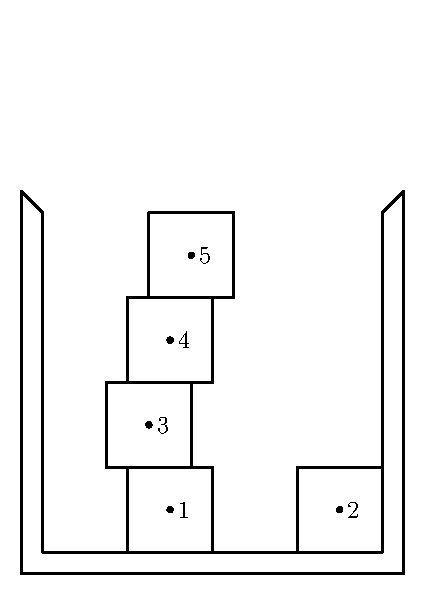
\includegraphics[width=\w]{btr-0}%
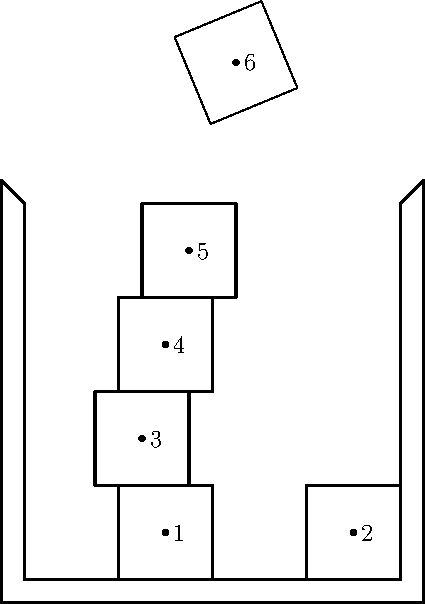
\includegraphics[width=\w]{btr-1}%
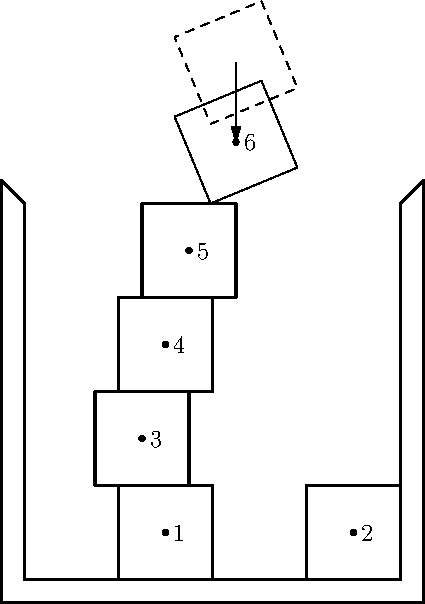
\includegraphics[width=\w]{btr-2}%
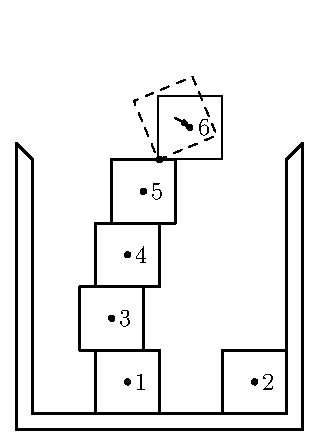
\includegraphics[width=\w]{btr-3} \\
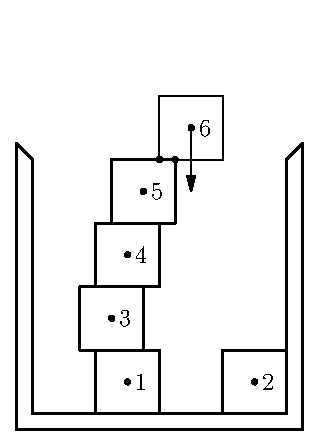
\includegraphics[width=\w]{btr-4}%
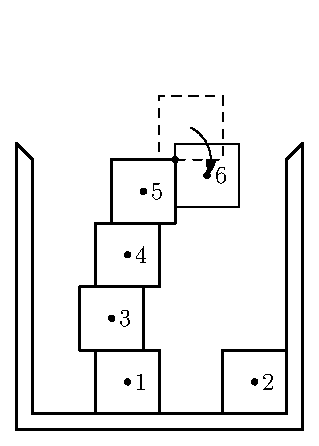
\includegraphics[width=\w]{btr-5}%
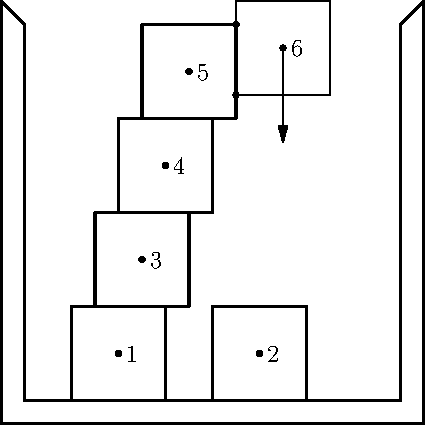
\includegraphics[width=\w]{btr-6}%
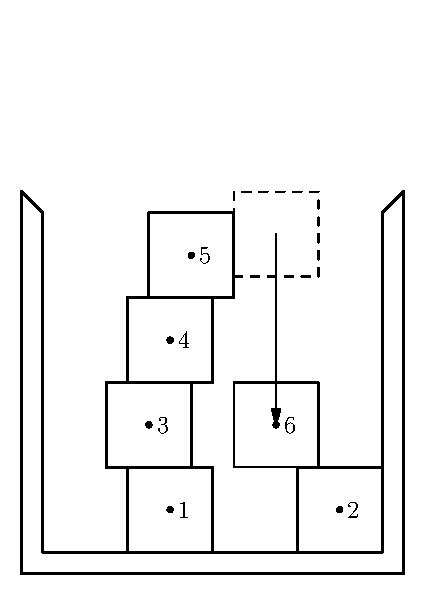
\includegraphics[width=\w]{btr-7} \\
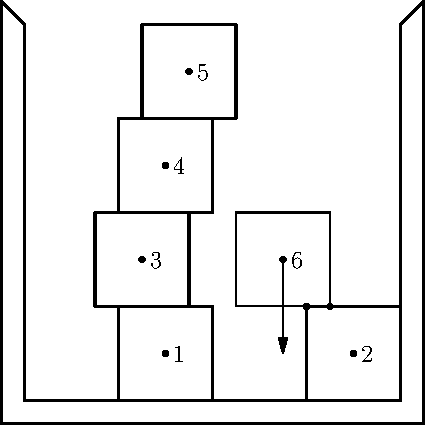
\includegraphics[width=\w]{btr-8}%
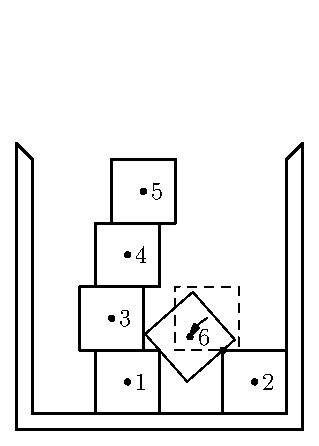
\includegraphics[width=\w]{btr-9}%
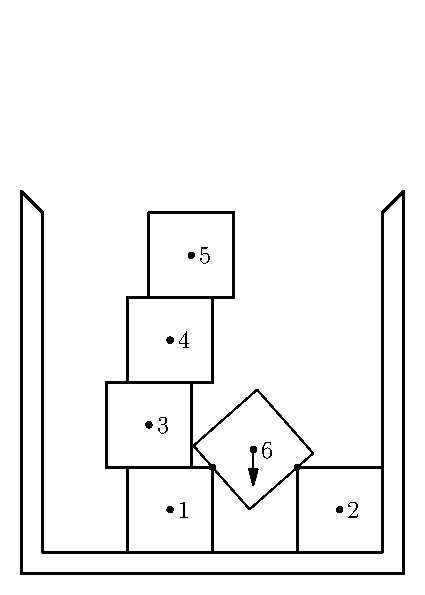
\includegraphics[width=\w]{btr-10}%
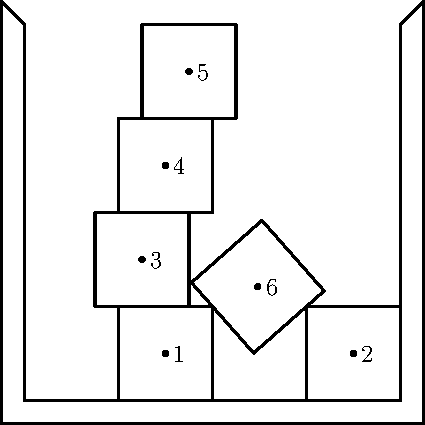
\includegraphics[width=\w]{btr-11}
\caption{Sketch of the bottom-to-top reconstruction algorithm.}
\label{f/btr}
\end{figure}

\begin{figure}
\centering
\def \w{0.25\columnwidth}
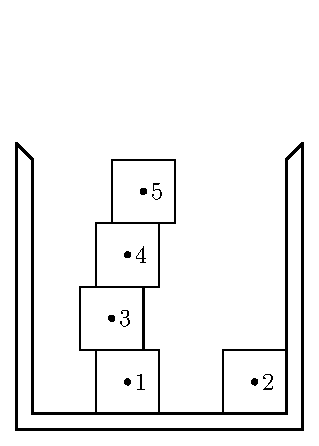
\includegraphics[width=\w]{dem-0}%
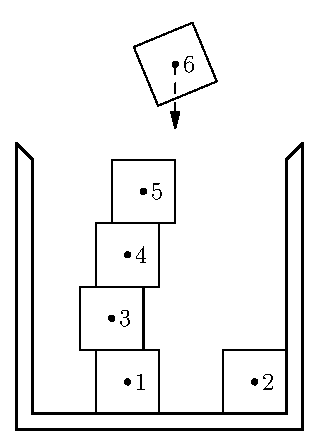
\includegraphics[width=\w]{dem-1}%
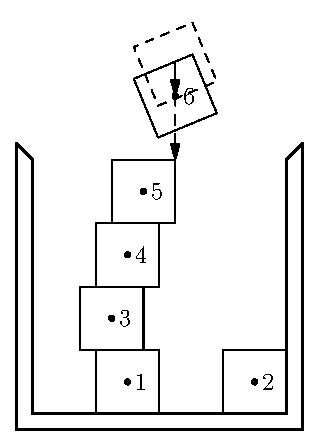
\includegraphics[width=\w]{dem-2}%
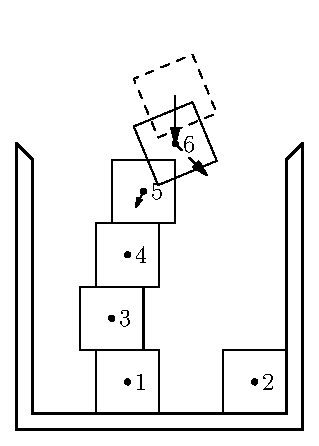
\includegraphics[width=\w]{dem-3} \\
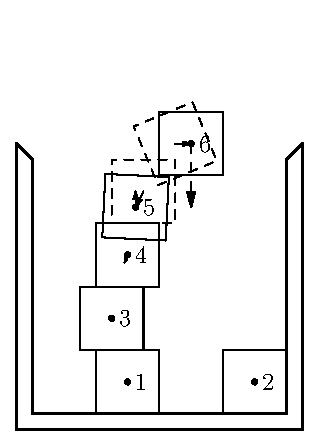
\includegraphics[width=\w]{dem-4}%
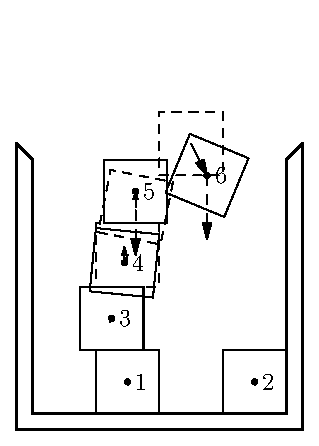
\includegraphics[width=\w]{dem-5}%
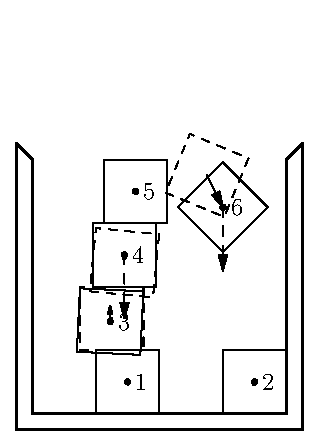
\includegraphics[width=\w]{dem-6}%
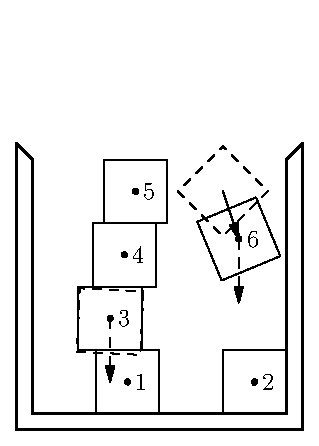
\includegraphics[width=\w]{dem-7} \\
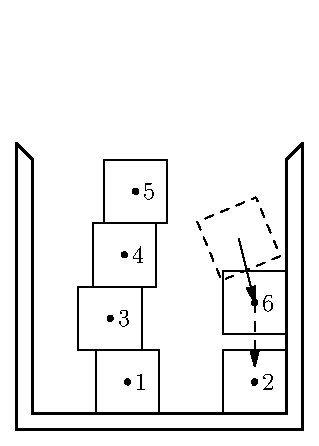
\includegraphics[width=\w]{dem-8}%
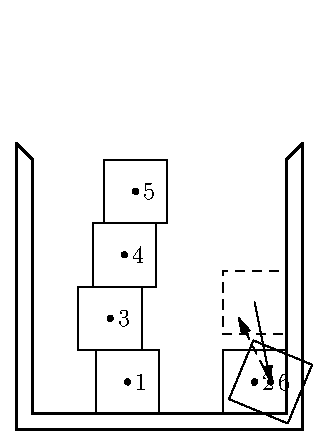
\includegraphics[width=\w]{dem-9}%
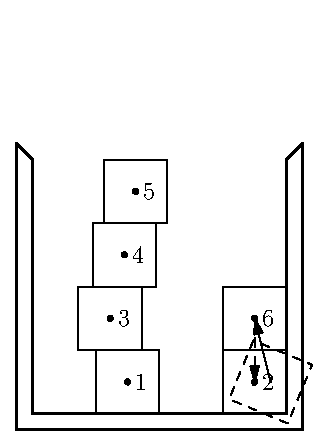
\includegraphics[width=\w]{dem-10}%
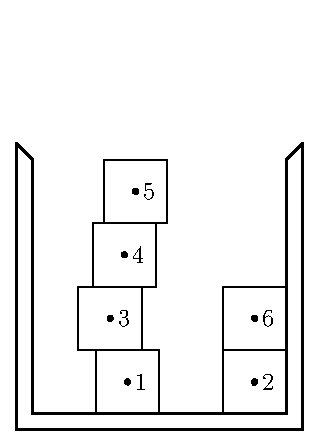
\includegraphics[width=\w]{dem-11}
\caption{Sketch of the force-based discrete element method.}
\label{f/dem}
\end{figure}

\subsection{Problem background}
The problem with storing random objects is encountered already in childhood as when cleaning one would have to put building blocks of different sizes and shapes in a box for storing. If individually organized little space will be wasted in the container and the lid of the box will most likely easily close. But saving time, most would not organize the blocks but just throw them in, and this poses an interesting problem, will the blocks fit inside the container so that the lid will close properly?
To study this question one would like to know what the packing density of the container is when the content is put in randomly.

The packing density is likely dependant on a variety of properties. Among other things the shape of the object put in it, the shape of the container and the sizes of the object, both in comparison to each other and to the container. When all objects are completely round is an well studied problem, therefore this report aims to study other shapes.
To simplify the problem, only objects of the same shape is considered, cubes. Further simplification is reducing from 3D to 2D, leaving the objects to be squares.
The assumption that the container will not move is made. When packing a box of randomly oriented objects that does not really fit, one would probably shake it to rearrange the configuration. This changes the problem and add complexity, it will therefor not be addressed.

%Discuss difficulties?
Originating from the solution with balls the biggest difference is that the orientation of the ball when it falls into the container does not affect the result. But for cubes, the orientation in all three dimensions matters, as ignoring it will lead to physically impossible configurations.

\subsection{Notes and Drafts}

We decided to start with a bottom-to-top reconstruction algorithm used
for granular dynamics (\cite{poschel-2005}),
but specialize it for rectangular particles.

\subsubsection{Bottom-to-Top Reconstruction}
First square will land on the bottom. If landing flat on one side, it is in a stable condition and the square is fixed at its position. If at all tilted when landing, only one corner of the square is supported which is not a stable state. It will therefor tilt in the direction of the center of mass, in the unlikely event that the center of mass is exactly above the supported corner, the direction doesn't matter. It will continue to tilt until it is stable which could happens in two ways. Either it falls on its side or it hits the wall of the container and stays tilted, supported by one point on the bottom and one on the container wall. This is also a stable state and it will thereafter stay fixed.
%Picture of possible outcomes, one square flat on bottom, one tilted against the wall?

Second square is the same procedure if not in contact with the first. Otherwise many possible outcomes occurs. If the first square is flat, landing with one side flat on the first square could be stable if the center of mass is inside the contact with the first square, if so it is fixed. If not the second square will tilt around the corner of the first square until another point is in contact with the wall or the sides of the squares are connected. It will then continue to tilt, still with the corner of the second square in contact with the side of the first. This will continue until it two points of contact is reached.
%Picture of tilting process?
If landing in contact with the flat first square with an angle it will behave as landing on the bottom, it will tilt in the direction of the center of mass. When having a flat contact it will behave as already described above.
When the first cube is not flat, but instead tilted against the wall, the same procedure as above is performed, tilting against the center of the mass. This might have to be done a few more times but the principle is the same.

Adding more squares is mostly repeating the same rules, with the difference that with more squares the landscape to which the squares are falling changes and more squares are in contact with each other leading to other possible stable states.



%What is the big picture (outline)?

\subsubsection{Line Intersection}

The intersection of two lines in a plane is easily obtained by solving
\begin{align*}
  X_1 + t_1 E_1 & = X_2 + t_2 E_2
  \yesnumber
\end{align*}
where $X$ are the positions (start vertices),
$E$ are the normalized direction vectors (vertex differences) and
$t$ are free.
If the lines are segments,
they intersect whenever $0 \le t_i \le 1$ for all $i$.
There also exists a three-dimensional generalization,
which yields the points,
where the two lines are the closest.

\subsubsection{Pivot Selection}

How to select the pivot?

\subsubsection{Rotation}

The rotation matrix around the origin
in the plane spanned by the first two dimensions is
\begin{align*}
  R (\theta) & =
  \begin{bmatrix}
    \cos \theta & -\sin \theta \\
    \sin \theta & \cos \theta
  \end{bmatrix}
  \yesnumber
\end{align*}
where $\theta$ is the angle.
In order to rotate around an arbitrary point,
we need to extend this to an affine transformation.
The familiar way is to use homogeneous coordinates.
We thus define the rotation matrix
\begin{align*}
  R' (\theta) & =
  \begin{bmatrix}
    \cos \theta & -\sin \theta & 0 \\
    \sin \theta & \cos \theta & 0 \\
    0 & 0 & 1
  \end{bmatrix}
  \yesnumber
\end{align*}
and the translation matrix
\begin{align*}
  T (x) & =
  \begin{bmatrix}
    1 & 0 & x_1 \\
    0 & 1 & x_2 \\
    0 & 0 & 1
  \end{bmatrix}.
  \yesnumber
\end{align*}
Composing them gives the matrix for a rotation around a point,
which we shall refer to as pivoting,
\begin{align*}
  P (x, \theta) & = T (x) R (\theta) T (-x).
  \yesnumber
\end{align*}

\subsubsection{Order Metrics}

In physics parlance,
quantitative ways to measure randomness
in a system are called order metrics.
There are various kinds (\cite{torquato-2002}).
Alas, most assume the system consists of point particles,
features bonds (chemical or otherwise) or
tends to arrange into a known set of crystal structures.
Our system does not have these properties,
so we cannot employ them directly.

The best option we could lift from physics is
the two-body excess entropy (\cite{truskett-2000}),
which has the dimensionless form
\begin{align*}
  \frac S{k^{\mathrm B}} & = -\frac 1 2 \Big(\frac N V\Big)
  \int_0^\infty \fulld r \big(g \log g - (g - 1)\big),
  \label{e/entropy} \yesnumber
\end{align*}
where $N$ is the number of particles,
$V$ is the total volume of the ambient space,
$g$ is the radial distribution function parametrized
by the distance $r$ (obtainable
through weighted kernel density estimation (\cite{kiiskinen-2018})) and
$k^{\mathrm B}$ is the Boltzmann constant.
However, this does not consider the orientation of the bodies.
To do that,
we could use the orientational correlation function (\cite{donev-2006}),
but it is not obvious how to incorporate it yet.

While the (unnormalized) radial correlation function says
\begin{align*}
  g_2 (r) & = \langle\delta (r - r')\rangle_{r'},
  \label{e/radial} \yesnumber
\end{align*}
the orientational correlation function
\begin{align*}
  g_m (r) & = \langle\cos m (\theta - \theta')\rangle_{\theta'},
  \label{e/angular} \yesnumber
\end{align*}
where $m$ is the degree of the symmetries as in (\cite{donev-2006}).
We conjecture that for squares $m = 4$ and for rectangles $m = 2$.
More is in (\cite{saintillan-2007}) and (\cite{stoyan-1991}).
Unfortunately combining these is not discussed anywhere.
This looks very promising (\cite{jiao-2011}).

\subsubsection{Why 2D Instead of 3D}

Proper collision prediction seems to be a hard problem,
as indicated by ``recent'' publications (\cite{kim-2003}).

\section{Instructor's assessment}

Every instructor is asked to add a brief (1--2 paragraph) summary of how the
group has performed through the week, especially with respect to the problem's
initial goals and the actual achievements. Here is also the place to report
possible total or part-time absences of the students during the group work
hours --- these can be also reported by the fellow group mates.

\clearpage

\thispagestyle{empty}
\addcontentsline{toc}{section}{References}

Possible references should be included in Harvard (author and year) style.

\printbibliography

\end{document}
